Во \underline{\textbf{второй главе}} представлены результаты исследования взаимное влияние ОМЧВС и ММЧВС при синхронном распространении мощных наносекундных импульсов накачки (1030~нм) и затравки (1562~нм) в маломодовом коммерчески доступном ОВ доставки FUD-3564~\cite{fud3564}. Данное ОВ поддерживает распространение двух поперечных мод ($\LPoi$, $\LPii$) на длине волны накачки и является одномодовым ($\LPoi$) на длине волны затравки. Длительность импульсов и частота их повторения составляет 2~нс и 5~МГц соответственно, величина пиковой мощности импульсов накачки и затравки равна 4~кВт и 0.5~кВт соответственно. %Показано, что оба процесса имеют общую антистоксову компоненту на длине волны 1003~нм, что приводит к перекрытию их спектров их коэффициентов усиления и взаимному влиянию процессов друг на друга. Экспериментально установлено, что синхронизация импульсов накачки и затравки увеличивает спектральную мощность компонент ММЧВС на 20 дБ, что ведёт к снижению эффективности последующей ГРЧ в н-о кристалле.

В главе показано, что в исследуемом ОВ доставки достигается взаимное влияние двух процессов ЧВС, развивающихся по следующим схемам:

\begin{equation}
	\LPoi^{1030}+\LPii^{1030}\longrightarrow \LPoi^{1003}+\LPii^{1059}
	\label{eq:synopsis_schemeIMFWM}
\end{equation}
\begin{equation}
	\LPoi^{1030}+\LPoi^{1562}\longrightarrow \LPoi^{1003}+\LPoi^{1629}	
	\label{eq:synopsis_schemeFWM}
\end{equation}

В~\cref{eq:synopsis_schemeIMFWM,eq:synopsis_schemeFWM} нижний индекс соответствует номеру поперечной моды, верхний индекс соответствует длине волны в нм.

Для подтверждения факта развития ММЧВС в ОВ проведён ряд экспериментов. На рис.~\cref{fig:synopsis_scheme_osa} показана схема эксперимента по определению спектрального состава излучения накачки, распространяющейся в поперечной моде $\LPii$.


\begin{figure}[h!]
	\centering
	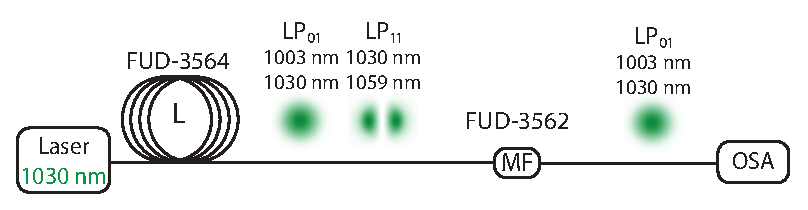
\includegraphics[width=0.8\linewidth]{Dissertation/images/imfwm/scheme_osa.eps}
	\caption{Блок-схема экспериментальной установки для определения спектрального состава излучения в поперечной моде $\LPii$. MF: модовый фильтр; OSA: анализатор спектра.}
	\label{fig:synopsis_scheme_osa}
\end{figure}

\begin{figure}[h!]
	\centering
	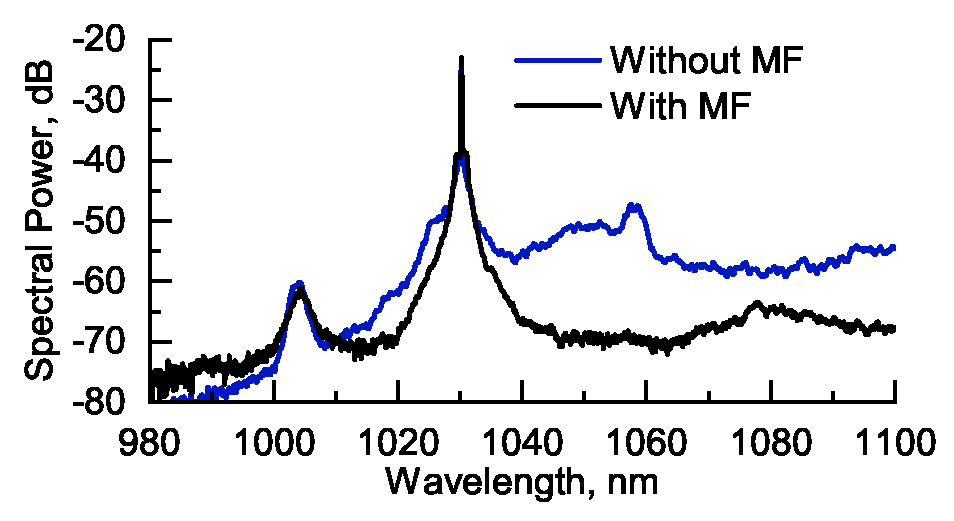
\includegraphics[width=0.55\linewidth]{Dissertation/images/imfwm/mode_filter_spectra}
	\caption{Спектры в области $1~\text{мкм}$ с применением (чёрный) и без применения (синий) МФ.}
	\label{fig:synopsis_mode_filter_spectra}
\end{figure}


На рис.~\cref{fig:synopsis_mode_filter_spectra} синяя и чёрная кривые соответствуют спектрам с модовым фильтром (МФ) и без него соответственно. МФ~--- это участок одномодового ОВ FUD-3562~\cite{fud3562}, согласованного по модовому диаметру с ОВ доставки. В спектральных областях $1030~\text{нм}$ (накачка) и $1003~\text{нм}$ (антистоксовая компонента) различия между спектрами минимальны, что указывает на сохранение этих компонент при распространении излучения через МФ. В спектральной области около $1059~\text{нм}$ (стоксовая компонента) МФ ослабляет излучение на $20~\text{дБ}$, что свидетельствует о присутствии моды $\LPii$ в данной спектральной области.


\begin{figure}[h!]
	\centering
	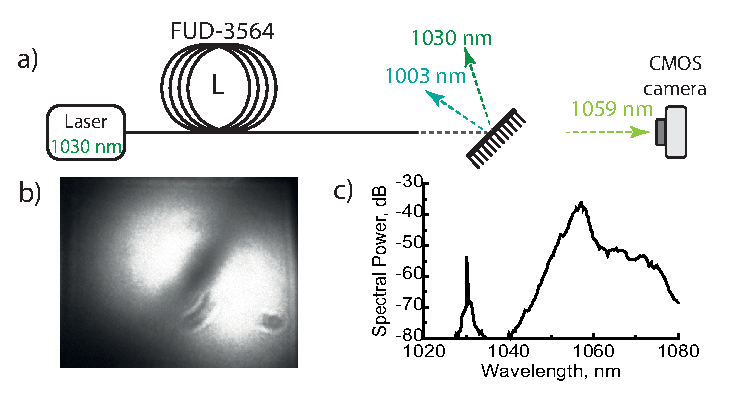
\includegraphics[width=0.8\linewidth]{Dissertation/images/imfwm/scheme_mirror.eps}
	\caption{a) Экспериментальная установка для визуализации пучка на длине волны $1059$~нм; b) изображение пучка на длине волны $1059$~нм; c) спектр после дихроичного зеркала.}
	\label{fig:synopsis_scheme_mirror_lp11_spectra}
\end{figure}


На рис.~\cref{fig:synopsis_scheme_mirror_lp11_spectra} показаны схема эксперимента по визуализации поперечного распределения интенсивности излучения в спектральной области 1059~нм, изображение пучка и его спектр. Для разделения спектральных компонент в области 1050--1070~нм использовалось дихроичное зеркало. Изображение пучка имеет двухлепестковую структуру, характерную для моды $\LPii$.


\begin{figure}[h!]
	\centering
	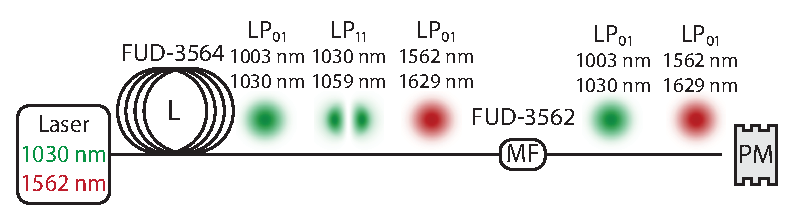
\includegraphics[width=0.8\linewidth]{Dissertation/images/imfwm/scheme_power.eps}
	\caption{Блок-схема экспериментальной установки для измерения доли оптической мощности моды $\LPii$. MF: модовый фильтр; PM: измеритель мощности.}
	\label{fig:synopsis_scheme_power}
\end{figure}

На рис.~\cref{fig:synopsis_scheme_power} представлена блок-схема эксперимента по демонстрации взаимного влияния ММЧВС в области 1 мкм и ОМЧВС между волнами накачки и затравки.

\begin{figure}[h!]
	\centering
	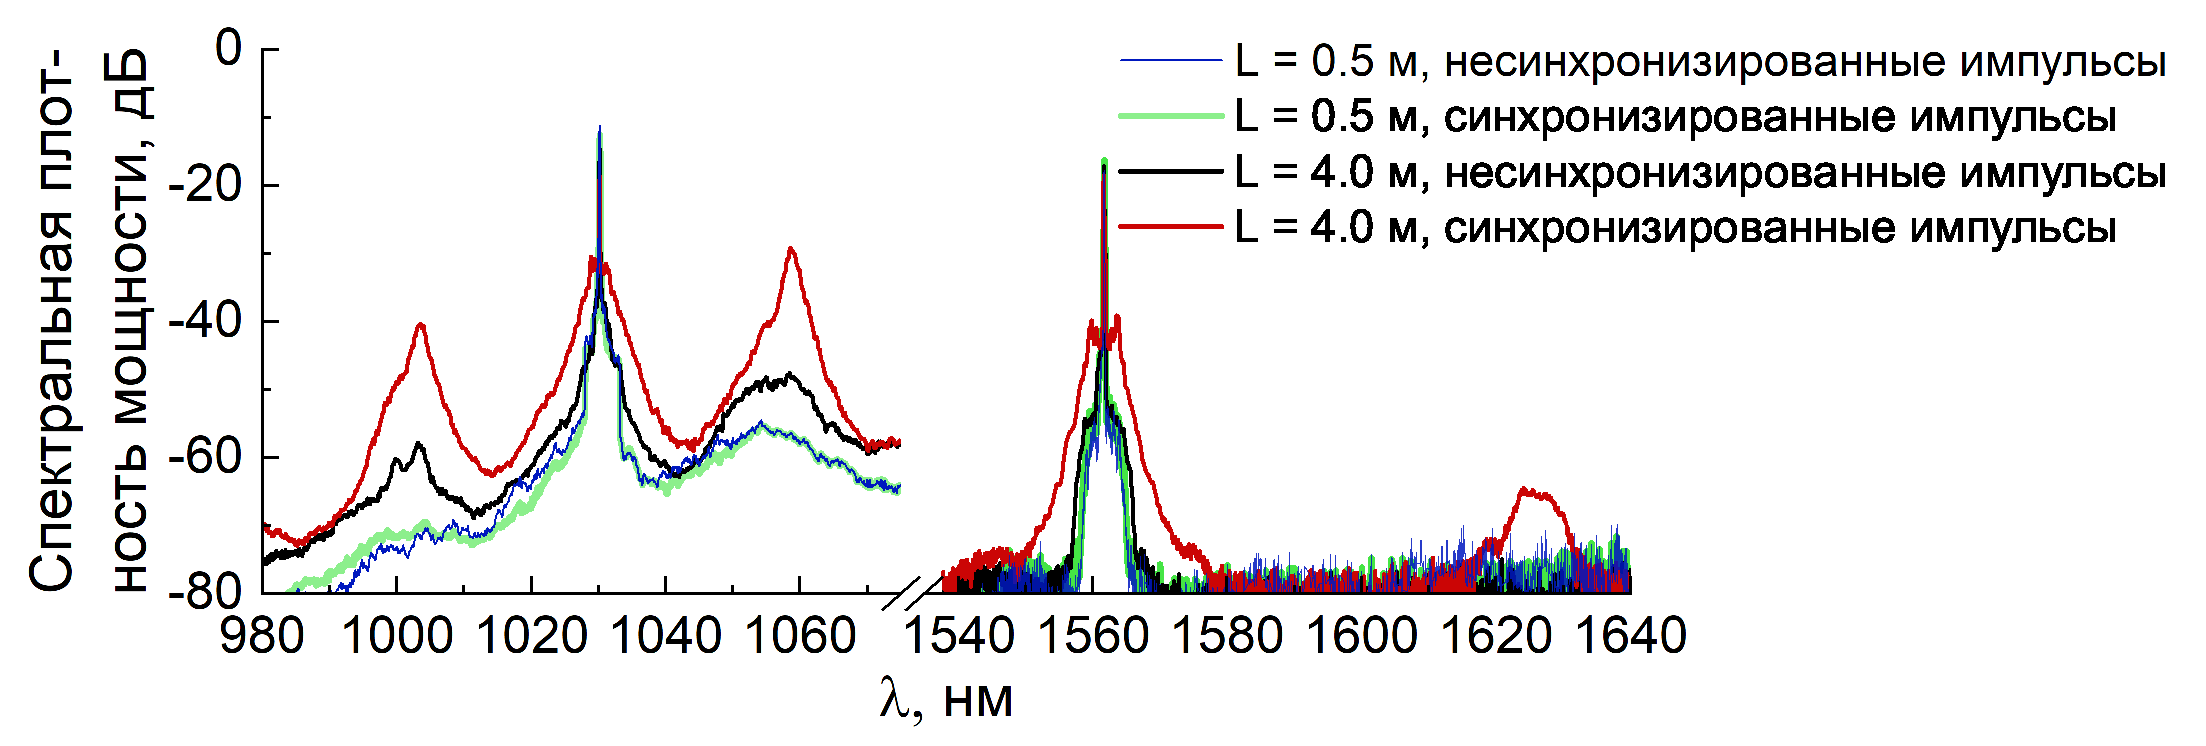
\includegraphics[width=0.85\linewidth]{Dissertation/images/imfwm/problem.eps}
	\caption{Измеренные спектры двухволнового лазера. L: длина ОВ}
	\label{fig:synopsis_problem}
\end{figure}

Из спектров, измеренных для синхронизированных и несинхронизированных импульсов (рис.~\cref{fig:synopsis_problem}) следует, что при распространении синхронизированных импульсов по ОВ доставки длиной 4~м на 20~дБ возрастает спектральная мощность как антистоксовой (1003~нм), так и стоксовой (1059~нм) компонент ММЧВС. Были измерены зависимости доли мощности моды $\LPii$ от длины ОВ доставки для случаев синхронизированных и несинхронизированных импульсов накачки и затравки. Показано, что синхронизация импульсов приводит к увеличению доли высшей моды при фиксированной длине ОВ.


\begin{figure}[h]
	\centering
	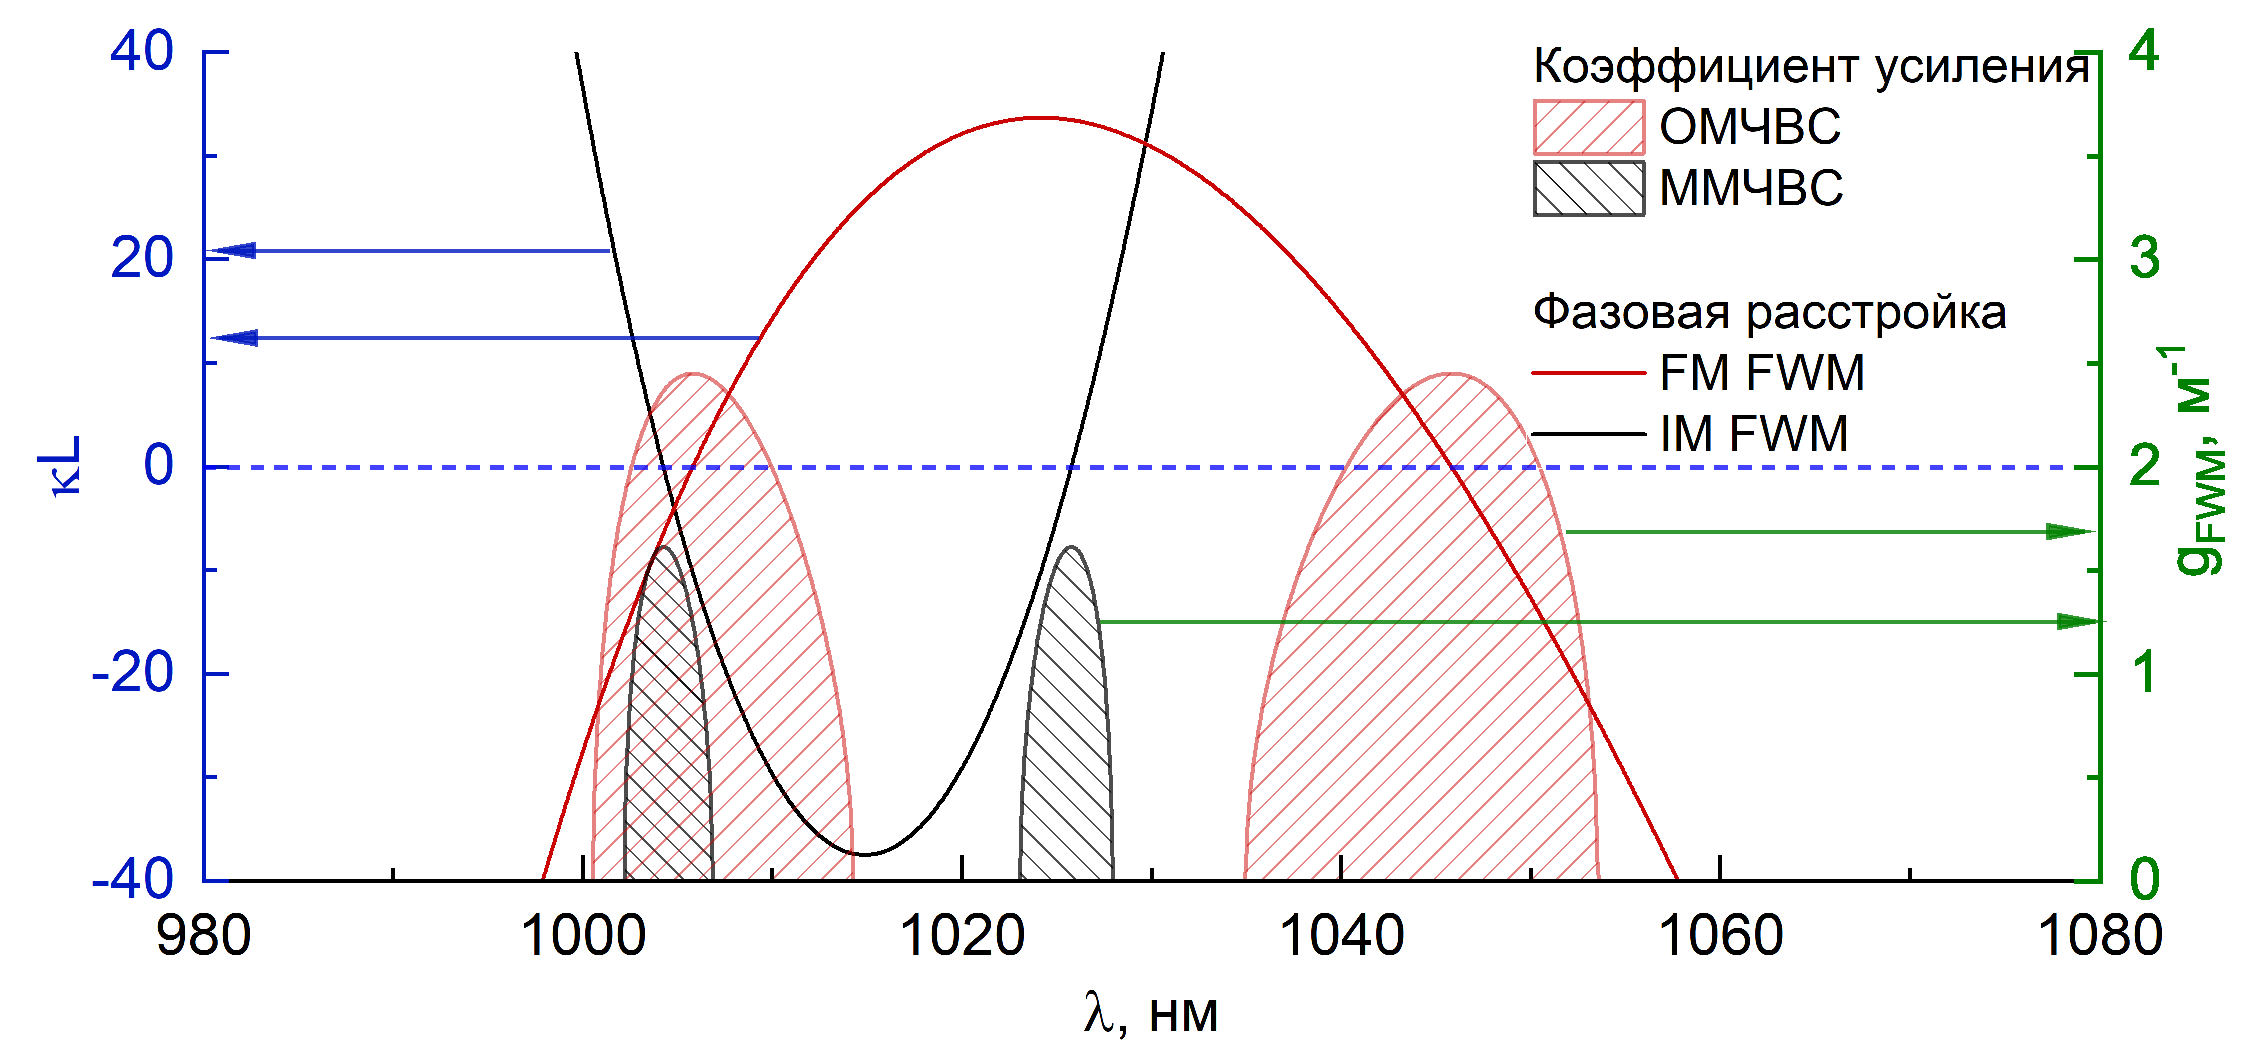
\includegraphics[width=0.8\linewidth]{Dissertation/images/imfwm/phase_sync_kappa.eps}
	\caption{Рассчитанная волновая расстройка (сплошные линии, левая шкала) и спектры усиления (штрихованные области, правая шкала) для ОМЧВС (красный) и ММЧВС (чёрный). Длина ОВ доставки: $L=4~\text{м}$.}
	\label{fig:synopsis_phase_sync}
\end{figure}


Экспериментальные результаты подтверждены теоретической моделью взаимодействия ОМЧВС и ММЧВС в ОВ доставки на основе системы связанных нелинейных уравнений распространения с учётом интегралов перекрытия поперечных мод~\cite{agrawal2019}. Для ММЧВС и ОМЧВС, (схемы~\cref{eq:synopsis_schemeIMFWM} и~\cref{eq:synopsis_schemeFWM}, соответственно), рассчитаны КФС и спектры коэффициента усиления $g_{\text{FWM}}$ (рис.~\cref{fig:synopsis_phase_sync}, сплошные линии и штрихованные области, соответственно). Оба процесса имеют общую антистоксовую компоненту на длине волны 1003~нм в моде $\LPoi$. Рассчитанные спектры излучения накачки и затравки, прошедших через ОВ доставки длиной 4~м (рис.~\cref{fig:synopsis_model_spectra}) показывают увеличение на 20~дБ спектральной мощности антистоксовой и стоксовой компонент ММЧВС при синхронизации импульсов, что соответствует экспериментальным результатам.

\begin{figure}[h]
	\centering
	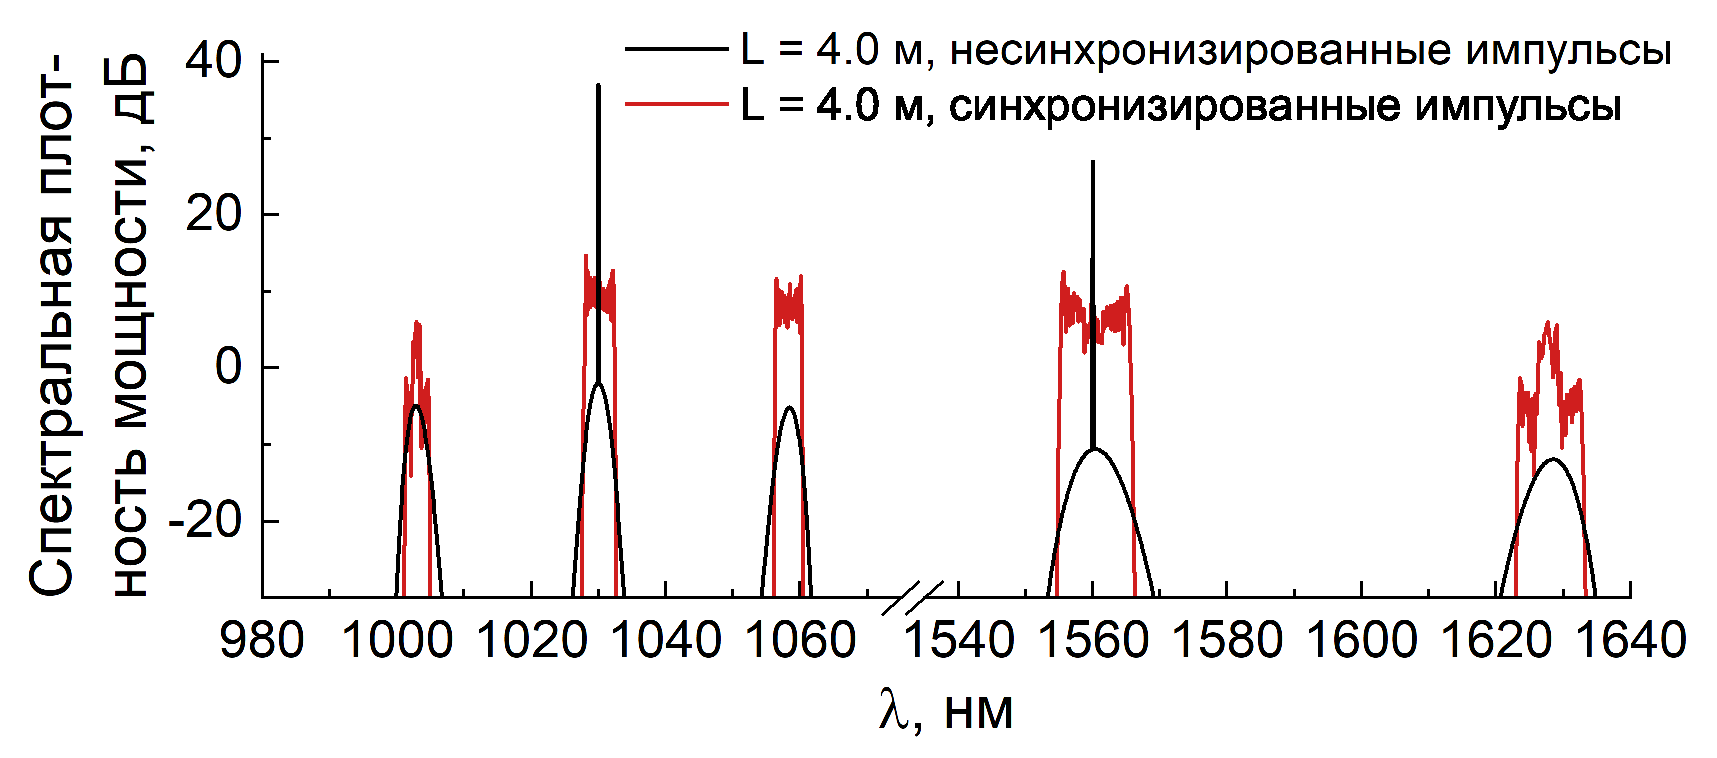
\includegraphics[width=0.7\linewidth]{Dissertation/images/imfwm/model_spectra.eps}
	\caption{Рассчитанные спектры двухволнового лазера для несинхронизированных (только ММЧВС, чёрный) и синхронизированных (ОМЧВС и ММЧВС, красный) импульсов}
	\label{fig:synopsis_model_spectra}
\end{figure}

Для подавления нежелательного взаимного влияния ОМЧВС и ММЧВС предложен метод, основанный на фильтрации высшей моды $\LPii$ на длине волны накачки с помощью МФ на входе ОВ доставки, что позволяет снизить её долю на входе ОВ с 15\% до $<0.4$\%. Наличие моды $\LPii$ на этой длине волны на входе ОВ доставки объясняется использованием маломодового активного ОВ в схеме лазера. Эффективность метода оценивалась по доле мощности моды $\LPoi$ в спектральном диапазоне $1030.0\pm0.5$~нм, определяющим эффективность последующей ГРЧ в н-о кристалле. При $L = 3$~м применение МФ на входе ОВ доставки уменьшает долю мощности моды $\LPii$ на его выходе на 30\%, сохраняя полезную мощность накачки. При $L = 4$~м подавление ММЧВС приводит к развитию вынужденного комбинационного рассеяния, что ограничивает эффективность метода. Согласно количественным оценкам, использование МФ повышает допустимую длину ОВ с 2.5 до 3.0~м без снижения эффективности последующей ГРЧ более чем на 10\% от максимального значения.